\chapter{Color Coding}
\label{cap 2}
Nel capitolo viene descritta la tecnica del Color Coding utilizzata in questa tesi.

La tecnica fu introdotta nel 1995 da Alon, Yuster e Zwick \cite{alon1995color}.
In generale, dato un grafo $G = (V,E)$, il problema dell'isomorfismo dei sottografi  di $G$ \`e un problema $NP$-completo.
Il metodo del Color Coding permette di risolvere sottocasi di questo problema in tempo polinomiale, tramite un algoritmo randomizzato.

Il primo algoritmo che loro descrissero, per\`o, si limitava alla ricerca di sottografi indotti in un grafo, senza farne un conteggio del numero delle occorrenze totali.
 
\`E per questo motivo che in questo capitolo si presenta un'estensione dell'algoritmo descritto da Alon \cite{alon1995color,bressan2018motif}, per effettuare un conteggio delle occorrenze dei treelet all'interno del grafo, che viene effettuato in maniera simultanea.
Dati in input un grafo $ G=(V,E) $ e un numero $ k $, per prima cosa il color coding assegna uniformemente e indipendentemente per ogni nodo di $ G $ un'etichetta in $ [k] := \{1,....,k\} $, indicato come un colore.
L'obiettivo \`e quello di conteggiare il numero di occorrenze di alberi colorati non indotti di $ k$-nodi in $ G $ - chiamati $ k-treelet $ - in cui ogni vertice dell'occorrenza ha un colore distinto.\\
Questo viene fatto in maniera efficiente mediante  programmazione dinamica, una tecnica che identifica dei sottoproblemi del problema originario, procedendo dai problemi pi\`u piccoli verso quelli pi\`u grandi.




\section{Algoritmo}
\label{section1}

In questa sezione viene descritta l'estensione dell'algoritmo del color coding che pu\`o contare i treelet (non indotti) colorati uniformemnte a caso.

L'algoritmo inizialmente prevede una fase di colorazione, dove ad ogni nodo $ v \in V $ di $ G $ \`e assegnato un colore $ c_v $, scelto indipendentemente e uniformemente a caso da $ [k] := \{1, \dots ,k\} $.\\
L'obiettivo della fase di costruzione \`e quello di creare una tabella con il conteggio delle occorrenze dei treelet che si possono incontrare in $ G $.\\
Per ogni nodo $ v \in V $ e per ogni albero colorato $ T_C $, con $ k $ nodi, si vuole calcolare il numero $ c(T_C , v) $ del numero di copie di $ T_C $  in $ G $ che sono radicate in $ v $ (si noti che qui si intendono copie non indotte).\\
Si pu\`o immaginare $ T_C $ come una coppia $ (T,C) $ dove $ C \subseteq {1,\dots,k} $.\\
Quello che si fa \`e per ogni nodo $ v $ si inizializza $ c(T_{C_0} , v) = 1 $, dove T \`e il treelet di 1 nodo e $ C_0 = \{c_v\} $.
Per ogni $ h = 2,\dots,k $ a turno, si considera ogni possibile albero radicato T di dimensione $ h $ e ogni possibile insieme di colori $ C \subseteq [k] $ con $ |C| = h $.\\
Quindi $ \forall v \in V$ di $ G $, si calcola come segue il numero $ c(T_C,v) $ di occorrenze dei treelet (non indotti) radicati in $ v $ isomorfi a $ T $ e i cui colori giacciono nell'insieme $ C $. Si divide idealmente $ T $ in due sottoalberi colorati unici $ T' $ di dimensione $ i $ con $ i = 1, \dots,h-1 $ e $ T'' $ di dimensione $ h-i $.
I due alberi saranno tali che  $ T'' $ \`e il sottoalbero radicato in uno dei figli della radice di $ T $ e $ T' $ \`e il sottoalbero di $ T $, radicato in $ r $ contenente $ |T| - |T''| $ nodi.\\
Per calcolare $ c(T_C,v) $ si analizza $ \forall v \in V $ di $ G $ l'insieme dei nodi $ u \in V $ tale che la coppia $ (u,v)\in E $.
Quindi si prendono  tutti i treelet colorati radicati in $ v $ isomorfi a $ T'_{C'} $ precedentemente calcolati e tutti i  treelet radicati in $ u $ isomorfi a $ T''_{C''} $.
Se $ C' \cap C'' = 0 $, si procede al conteggio delle occorrenze di $ T_C $ radicato in $ v $ nel modo seguente:

\begin{equation}\label{conta}
	c(T_c,v)=\frac{1}{\beta_T}\sum_{(u,v)\in E}\sum_{\substack{C' \subset C \\C'' = C \setminus C' \\ |C'|=|T'|, |C''| = |T''|}}c(T'_{C'},v)\cdot c(T''_{C''},u)
\end{equation}

dove $ \beta_T $ \`e una costante di normalizzazione che \'e uguale al numero di alberi di $ T $ isomorfi a $ T'' $ radicati in un figlio di $ r $.\\
 La correttezza e la complessit\`a di questa costruzione, non sono trattate qui, ma vengono dimostrate in \cite{alon1995color}.\\
 Si pu\`o vedere l'algoritmo formalmente  descritto in Algoritmo \ref{algoritmo}.\mbox{}\\


\begin{algorithm}[H]
	\label{algoritmo}
	\SetAlgoLined
	\caption{Fase di costruzione}
 	\textbf{input} : Grafo $ G =(V,E) $, dimensione del treelet $ k $ \;	
 				\For{$ v $ in $ G $}{
 				$C_0 = \{c_v\}$; viene assegnato un colore uniformemente a caso preso da [$ k $]\;
 				$ c(T_{C_0} , v) = 1 $\;
 			}	
 			\For{$ h = 2$ to $ k $}{
 				\For{$ v \in V $}{
 					\ForEach{$ T : |T| = h $}{					
 						\( 	c(T_C,v)=\frac{1}{\beta_T}\sum_{(u,v)\in E}\sum_{\substack{{C',C''\subset C}\\{C'\cap C'' =0}}}c(T'_{C'},v)\cdot c(T''_{C''},u) \)	
 					}
 				}
 			}
 			
\end{algorithm}\mbox{}\\

Come si pu\'o notare, per calcolare le occorrenze di un albero $ T_C $ nell'algoritmo si sfrutta un approccio top-down, ossia a partire dall'albero $ T_C $ si identificano i due alberi $ T' $ e $ T'' $ in cui pu\`o essere scomposto, si considerano tutte le partizioni di $ C',C'' \subset C $ e in seguito si procede al calcolo di $ c(T_C,v) $ come indicato in \eqref{conta}.

In questa tesi, cos\'i come in \cite{bressan2019motivo}, invece, si \`e sfruttato un approccio bottom-up. Infatti, per ogni nodo $ v \in V $ di $ G $ e per ogni nodo $ u \in adj(v)$, si prendono tutte le coppie possibili di treelet colorati radicati rispettivamente in $ u $ e $ v $, $ T'_{C'} $ e $ T''_{C''} $, tali che $ |T'| + |T''| = k $ e $ |T'|,|T''|>0 $.

Dallo sviluppo dell'algoritmo \ref{algoritmo}, si noti che conteggia e salva per ogni nodo $ v\in V $ di $ G $ il numero di occorrenze di ogni $ k $-treelet colorati che si pu\`o raggiungere a partire da $ v $.
Lo scopo di questa tesi per\`o \'e quello di conteggiare il numero di $ k $-treelet colorati individuabili su tutto il grafo $ G $ e le occorrenze totali per ognuno.
A tale scopo \`e neccessario aggregare gli alberi in un unica tabella contenente i $ k $-treelet e le rispettive occorrenze.
Per evitare di conteggiare gli alberi un numero di volte superiori a quelle effettive, vengono classificati secondo una classe di equivalenza di isomorfismo. Dati due alberi $ T' $ e $ T'' $ si dicono isomorfi se esiste una funzione bijettiva $ f : T' \rightarrow T'' $.
Perci\`o se due alberi sono isomorfi, verranno raggruppati nella stessa classe di equivalenza e le loro occorrenze saranno sommate.
Cos\`i facendo otterremo i conteggi effettivi di tutti i $ k $-treelet trovati in $ G $ e il numero di volte che occorrono. 


\section{Dettagli implementativi: rappresentazione compatta dei treelet colorati}
\label{section 2}
In questa sezione vengono descritte le strutture dati usate per implementare l'algoritmo in Java.
Gli oggetti principali che vengono manipolati sono i treelet colorati e le occorrenze associate.

Ogni treelet colorato $ T_C = (T,C) $ ha una rappresentazione unica, nella quale sono memorizzate la topologia di $ T $, i colori in $ C $, ed informazioni aggiuntive per facilitare la minipolazione di $T_C$.
Tale rappresentazione richiede al pi\`u 59 bit e pu\`o pertanto essere memorizzata usando degli interi a 64 bit, un tipo di dati nativo in Java e nelle pi\`u comuni architetture moderne.
I bit sono numerati da 0 a 63 e ordinati dal bit meno significativo a qullo pi\`u significativo.\\
Sono cos\'i suddivisi:
\begin{itemize}
	\item i bit da 0-3 contengono il numero di nodi di $ T $ a meno della radice, che non \`e necessaria ai fini delle operazioni effettuate.
	\item i bit da 4-7 contengono la dimensione del sottoalbero radicato nell'ultimo figlio della radice di $ T $.
	\item i bit da 8-11 vengono usati per memorizzare il valore di $ \beta_T $ associato a $ T $.
	\item i bit da 12-27 sono usati per indicare i colori in $ C $
	\item i bit da 28-58 sono usati per codificare la struttura del treelet, come descritti nel seguito.
	\item gli ultimi 5 bit sono lasciati a zero
\end{itemize}\mbox{}\\

Per codificare la struttura dell'albero si procede nel seguente modo.\\
Si esegue una visita DFS su $ T $ partendo dalla radice $ r $ e attraversando gli archi di $ T $, in modo che, al termine della visita, ogni arco sia stato attraversato esattamente 2 volte, in direzioni opposte. 

Sia $h=|T|$ e sia $e_i$, con $i = 1, 2, \dots, 2(h-1)$, l'$i$-esimo arco attraversato dalla visita. 
L'$i$-esimo bit della codifica \`e $0$ se $e_i$ \`e attraversato in direzione di $r$ in $T$ e $1$ in caso contrario. In Figura \ref{figura} si pu\`o vedere un esempio di tale codifica.

\begin{figure}[htbp]
	\centering
	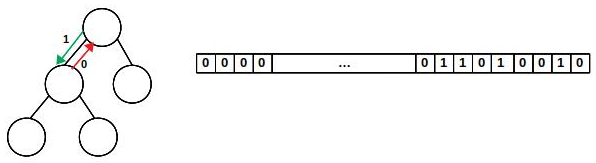
\includegraphics[width=11cm]{capitolo2/grafo3}
	\caption{Un treelet radicato e la codifica della sua struttura}
	\label{figura}
\end{figure}

Per un qualunque $ k \le 16 $ questa codifica richiede al massimo 30 bit.
L'ordinamento lessicografico sulla struttura permette anche un'ordinamento totale sui treelet. Questo ordinamento \`e anche una regola decisiva per la visita DFS: i figli di un nodo vengono visitati nell'ordine dato dai sottoalberi radicati in esso.
Ci\`o implica che ogni treelet $ T $ ha una codifica unica , ed ogni codifica valida corrisponde ad un solo treelet. Inoltre, in questo modo \`e possibile implementare rapidamente l'operazione di unione.\\

La codifica dei treelet supporta le seguenti operazioni :
\begin{itemize}
	\item $ \textbf{singleton} $ (c) : permette di inizializzare un treelet di un solo nodo con il rispettivo $ c \in {1, \dots, k} $
	\item $ \textbf{merge} $ ($ T' $,$ T'' $) : fa l'unione di due alberi $ T' $ e $ T'' $, se possibile creando un nuovo albero $ T $ che avr\`a come struttura la concatenazione delle strutture di $ T' $ e $ T'' $.
	Come dimensione, a meno della radice, $ T $ avr\`a la somma delle dimensioni di $ T' $ e $ T'' $ pi\'u 1, ossia il nodo radice di $ T'' $.
	I colori di $ T $, sono dati dall'unione dei colori di $ T' $ e $ T'' $.
	In $ T $ come $ \beta $ viene memorizzato il valore corrispondente a quello di $ T' $ e se la struttura del sottoalbero pi\'u piccolo di $ T' $ \`e uguale a quella di $ T'' $ viene incrementato di 1. Per finire, la dimensione del sottoalbero pi\`u piccolo radicato in $ T $ sar\`a esattamente la dimensione di $ T''+1  $ .
	\item $\textbf{normalization\_factor}$ ($ T $): restituisce la costante di normalizzazione $ \beta_T $ associata a $ T $.
	    
\end{itemize}
\begin{figure}[htbp]
	\centering
	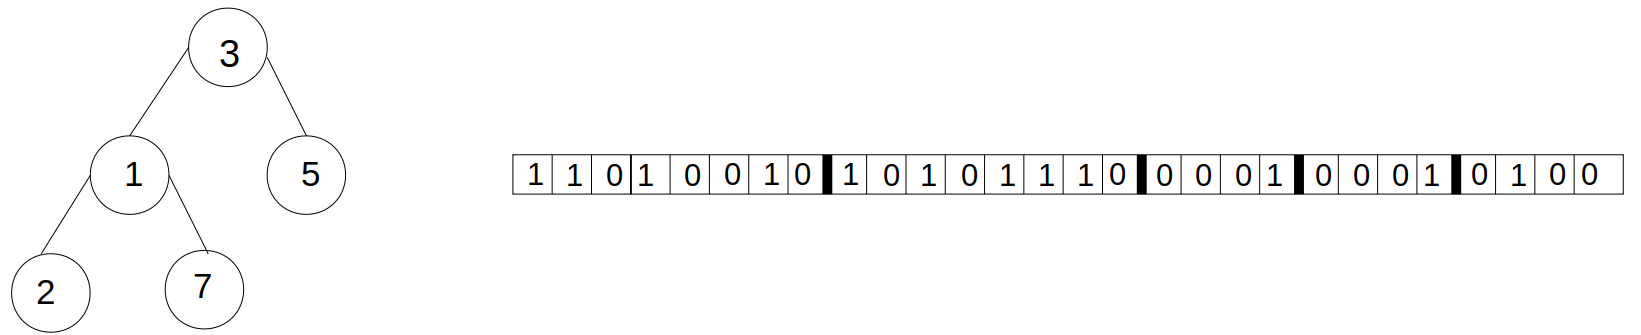
\includegraphics[width=11cm]{capitolo2/grafo4}
	\caption{un treelet colorato e la sua codifica, mostrata per semplicit\`a solo su 8+8+4+4+4=28 bit}
	\label{figura1}
\end{figure}
Un esempio di treelet colorato e della sua codifica \`e mostrato in Figura \ref{figura1}.\mbox{}\\\\
Nell'implementazione i treelet individuati da ogni nodo e i rispettivi conteggi vengono salvati all'interno di una tabella indicizzata, rappresentata mediante strutture annidate di $ ArrayList $.
Inizialmente come nell'algoritmo \ref{algoritmo} i treelet e i conteggi sono calcolati su ogni nodo $ v \in V $ di $ G $ scorrendo tutti gli archi $ E $.
Solo una volta calcolati  tutti i treelet su tutti i nodi $ v $, questi verranno aggregati e i loro conteggi sommati, inoltre per ogni classe di equivalenza sar\`a identificato un unico rappresentante che \`e il k-treelet radicato nel centroide.
Nella sezione \ref{section3} verr\`a data la definizione di centroide di un albero e l'algoritmo per la sua ricerca.\\
Inizialmente, perci\`o, quello che si ha \`e una tabella con $ k $ entrate, indicizzate da $ 1 $ a $ k $ ed associate al numero di vertici dei treelet.\\
L'$ i $-esima entrata della tabella, con $ 1\le i \le k $ generico, a sua volta, \`e un $ ArrayList $, con una dimensione fissata, che varia a secondo della cardinalit\`a di $ V $, cos\`i che ad ogni entrata \`e associato un vertice $ v\in V $ di $ G $.\\
Per ognuna delle $ |V| $ entrate, viene creato un $ ArrayList $ contenente tutti i treelet colorati di dimensione $ i $ raggiungibili dai differenti nodi in $ V $, insieme al relativo numero di occorrenze.\\
All'interno di quest'ultima lista i treelet sono ordinati in ordine non descrescente.\\
La tabella ha una costruzione dinamica, perci\`o l'$ i $-esima entrata \`e costruita solo dopo aver terminato la costruzione della $ i-1 $-esima.

Per permettere una costruzione pi\`u rapida della tabella, nell'implentazione \`e utilizzato il $ Multithreading $, cio\`e vengono utilizzati pi\`u thread che lavorano in parallelo.
Un thread \`e un flusso di esecuzione indipendente all'interno di un processo.
Il numero di thread utilizzato nell'implementazione \`e dipendente dal numero di processori presenti nella macchina.
Supponendo di avere un pc con 4 processori, vengono usati 3 thread, uno in meno rispetto al numero di processori.
Per garantire un funzionamento in parallelo senza conflitti \`e dovuto provvedere affinch\`e nessuna operazione necessitasse di semafori di mutua esclusione (mutex) e che ogni tipo di dato coinvolto fosse atomico, ossia non scomponibile.\\
Riguardo le operazioni sugli ArrayList non \`e stato necessario ricorrere alla mutua esclusione.
Per le variabili \`e stato necessario, invece, garantire la visita dei vertici del grafo in maniera atomica e a tal proposito i vertici, in ogni ArrayList, sono rappresentati mediante $ AtomicInteger $, ossia valori interi che possono essere aggiornati in maniera atomica.\mbox{}\\



	
